 
% Para una visualizacion correcta, generar el PDF
% Ni el DVI ni el PS se visualizan bien

% Elegir el estilo que se desee, hay cientos en la red

\documentclass{beamer}
\usepackage{beamerthemeshadow}
\usepackage{verbatim}
\usepackage{pgfpages}
\usepackage[galician]{babel}
%\usepackage[spanish]{babel}
\usepackage[utf8]{inputenc}
%\usepackage[latin1]{inputenc}
\usepackage[spanish,linesnumbered,lined,boxed,commentsnumbered,noend]{algorithm2e}
\usepackage{pgf-pie}

\setcounter{tocdepth}{1}% Allow only \chapter in ToC
\setbeameroption{show notes on second screen}
\setbeamertemplate{headline}{}


\begin{document}
\title[Intelixencia Artificial aplicada a Videoxogos Top-Down]{Intelixencia Artificial aplicada a Videoxogos Top-Down en tempo real}
\subtitle{Grao en Enxeñaría Informática \\
Universidade de Santiago de Compostela}  
\author{Autor: Rubén Osorio López}
\institute{Titor: Manuel Mucientes Molina\\Cotitor: Pablo Rodrígez Mier}
\date{21 de xullo de 2017} 

\begin{frame}
\titlepage
\note{Esto é a defensa da memoria do traballo de fin de grado nombrado \textbf{Intelixencia Artificial aplicada a Videoxogos Top-Down en tempo real}, eu son o autor, Rubén Osorio López, e os tutores son Manuel Mucientes Molina e Pablo Rodrígez Mier}
\end{frame}

\begin{frame}
\frametitle{Táboa de contidos}\tableofcontents
\note{Durante esta presentación seguiremos unha estructura similar á memoria, centrándonos máis en alguns aspectos concretos do proxecto que expliquen en que consistiu o traballo realizado.}
\end{frame} 



\section{Introdución} 

\begin{frame}
\frametitle{Introdución} 


	\begin{itemize}
		\item Proxecto que aborda a creación dun \textbf{videoxogo} con necesidades de \textbf{comportamento complexo} por parte do inimigo.
	\end{itemize} 

\begin{block}{Videoxogo}
	\textbf{Loita 1 contra 1}, \textbf{Top-Down} en \textbf{dúas dimensións}
\end{block}

\begin{block}{Axente}
Capaz de percibir e actuar sobre o \textbf{entorno competitivo} do videoxogo mediante \textbf{sensores} e \textbf{actuadores}
\end{block}
\note{
	
	De forma xeral, búscase a creación dun videoxogo que requira un inimigo con comportamento complexo. O axente que representará o inimigo necesita ser un competidor capaz, para o que se realizou unha etapa de entrenamento na que optivo a información que necesitaba.\\
	
	\textbf{Loita 1 contra 1} significa que soamente dous perxonaxes competirán entre eles contando ambos coas mesmas capacidades, accións posibles e atributos. \textbf{Top-Down} refírese ó plano picado utilizado para visualizar o combate. Por outra parte que sea en \textbf{dúas dimensións} implica que todo o contido do videoxogo son imaxen planas debuxadas unha a unha, sen que existan modelos en tres dimensións.\\
	
	\textbf{Un axente} é aquilo capaz de percibir o entorno mediante \textbf{sensores} e actuar sobre o mesmo en consecuencia mediante \textbf{actuadores}, ambos son proporcionados pola súa interface co videoxogo. Ademáis atoparase nun entorno competitivo o que implica que buscará maximizar o seu \textbf{rendemento} mentres se minimiza o do contrincante.
	


}
\end{frame}




\subsection{Obxectivos}
\begin{frame}
\frametitle{Obxectivos} 
\begin{itemize}
	\pause
	\item Implementación do videoxogo \pause
	\item Implementación do axente \pause
	\item Realizar o adestramento do axente \pause
	\item Obter datos sobre as capacidades do axente \pause
	\item Analizar os resultados obtidos
\end{itemize}
\note{
	\begin{itemize}
		\item Implementación do videoxogo: Xa que necesitaremos unha plataforma que nos permita que o axente e o xogador interactúen seguindo unha serie de regras comúns para competir entre eles.
		\item Implementación do axente: Necesitarase implementar o axente capaz de desenvolverse correctamente durante a competición.
		\item Realizar o entrenamento do axente: O axente necesitará obter a información necesaria para logo comportarse adecuadamente gracias ó aprendido durante a etapa de entrenamento.
		\item Obter datos sobre as capacidades do axente: Obteránse datos sobre o rendemento do axente contra outras implementacións máis sinxelas.
		\item Analizar os resultados obtidos: Coa información obtida durante todo o proxecto, e especialmente na etapa anterior, realizarase un análise que describa o que conseguiu o axente.
\end{itemize}
}
\end{frame}


\section{Videoxogo baseado en axentes}

\subsection{Mecánicas}
\begin{frame}
\frametitle{Mecánicas}

\begin{block}{Movemento}
Movemento libre nunha habitación rectangular.
\end{block}

\begin{block}{Ataque}
Permítese atacar a zona que se atopa cada onde o personaxe está mirando.
\end{block}

\begin{block}{Defensa}
Posibilidade de defenderse dun ataque permitindo atacar se a defensa ten éxito
\end{block}

\note{
\textbf{Movemento} libre nunha habitación rectangular que suma a complexidade de evitar situacións nas que non se poida escapar do contrincante por estar ó lado dunha parede ou unha esquina. Ademáis a única maneira de mirar cara unha dirección é mirar cara ela.\\
\textbf{Como} solo se permite atacar a zona directamente enfrente do personaxe é importante ter en conta cada donde se está mirando. Esto favorece unha actitude agresiva pois hai que moverse na dirección do enemigo antes de atacalo.\\
\textbf{Pódese} realizar unha maniobra defensiva de alto risco e alta recompensa que permite evitar un ataque. Se se evita con éxito poderase realizar un ataque propio pero se non serase vulnerable durante uns instantes.\\
\textbf{Esto fai que non exista unha estratexia idónea} pois un estilo agresivo perde contra un defensivo que á sua vez perde contra xogadores que busquen a contra do movemento defensivo, este último ademáis perde contra o xogador agresivo. Esta fórmula de \textbf{pedra, papel, tesoiras} demostrou ser ampliamente utilizada en diseño de videoxogos.\\
}
\end{frame}


\subsection{Prototipo de Unity}
\begin{frame}
\frametitle{Prototipo de Unity}
Primeira implementación realizada con \textbf{Unity3D}, estándar de facto para videoxogos de este tamaño.
	\vspace{0.5cm}
\begin{alertblock}{Problemas de simulación}
	Imposibilidade de escalar o tempo sen romper o funcionamento do videoxogo.
\end{alertblock}
\note{
\textbf{Ensinar vídeo}
}
\end{frame}


\subsection{Segunda aplicación}
\begin{frame}
\frametitle{Segunda aplicación}
Implementación de un motor desde cero en C++

\begin{figure}
	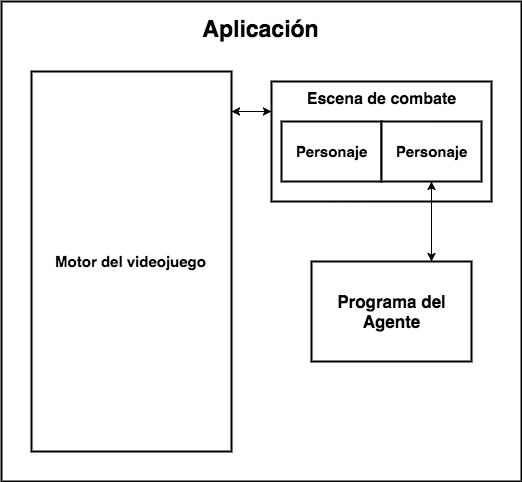
\includegraphics[scale=0.3]{../otros/otrasCapturas/block.png} 
\end{figure}

\note{
	
}
\end{frame}

\subsection{Algoritmo}
\setlength{\algomargin}{0.11cm}
\begin{frame}
\frametitle{Algoritmo}
\begin{center}
	\scalebox{0.55}{
		\begin{minipage}{1.2\linewidth}
			\begin{algorithm}[H]
				\SetKwData{Action}{action}
				\SetKwData{LastAction}{selectedAction}
				\SetKwData{LastState}{lastState}
				\SetKwData{CurrentState}{currentState}
				\SetKwData{DeltaFitness}{deltaFitness}
				\SetKwData{StateActionData}{stateActionData}
				\SetKwData{RandomAction}{randomAction}
				\SetKwData{AllActions}{allPosibleActions}
				
				\SetKwFunction{GetRandomAction}{getRandomAction}
				\SetKwFunction{GetCurrentState}{getCurrentState}
				\SetKwFunction{RandomBet}{randomBetween}
				\SetKwFunction{CalculateFitness}{calculateFitness}
				\SetKwFunction{UpdateWith}{updateWith}
				\SetKwFunction{Insert}{insert}
				\SetKwFunction{Pick}{bestWeightedAction}
				
				\While{agent is running}{
					\LastState$\leftarrow$ \CurrentState\;
					\CurrentState$\leftarrow$ \GetCurrentState{}\;
					
					\DeltaFitness$\leftarrow$ \CalculateFitness{\CurrentState}$-$\CalculateFitness{\LastState}\;
					
					%Actualizamos el conocimiento del agente
					\uIf{\LastState$\in$ \StateActionData}{
						\StateActionData$.$\UpdateWith{\LastState,\LastAction,\DeltaFitness}\;
					}
					\Else{
						\StateActionData$.$\Insert{\LastState,\LastAction,\DeltaFitness}\;
					}
					
					
					%Seleccionamos la acción a escoger
					\uIf{\CurrentState$\in$ \StateActionData}{
						
						\uIf{\RandomBet{$0$,$1$}$<\epsilon$}{
							\LastAction$\leftarrow$ \RandomAction $\in$ \AllActions\;
						}
						\Else{
							\LastAction$\leftarrow$ \Action $\in$ \AllActions  $|$ \Pick{\StateActionData,\CurrentState} $=$ \Action  \;
						}
						
					}
					\Else{
						\LastAction$\leftarrow$ \RandomAction $\in$ \AllActions\;
					}
					
					
				}
				\label{algoritmo}
			\end{algorithm}
		\end{minipage}%
	}
\end{center}


\note{
	
}

\end{frame}

\begin{frame}
\frametitle{\textit{Fitness}}


\begin{columns}
	\begin{column}{5cm}
\begin{center}
	\scalebox{0.5}{
		\begin{minipage}{1.6\linewidth}
			\begin{algorithm}[H]
					\SetKwData{Fitness}{fitness}
				
				\SetKwData{PlayerHealth}{playerHealth}
				\SetKwData{EnemyHealth}{enemyHealth}
				\SetKwData{Distance}{distance}
				\SetKwData{LookingAtEnemy}{lookingAtEnemy}
				\SetKwData{NoWallsNear}{noWallsNear}
				
				\SetKwFunction{GetRandomAction}{getRandomAction}
				\SetKwInOut{Input}{input}\SetKwInOut{Output}{output}
				\Input{\PlayerHealth, \EnemyHealth, \Distance, \LookingAtEnemy, \NoWallsNear}
				\Output{\Fitness}
				
				
				\Fitness$\leftarrow$ INITIAL\_FITNESS\_VALUE\;
				\Fitness$\leftarrow$ \Fitness$+ ($\PlayerHealth$*$ MY\_HEALTH\_MULTIPLIER$)$\;
				\Fitness$\leftarrow$ \Fitness$- ($\EnemyHealth$*$ ENEMY\_HEALTH\_MULTIPLIER$)$\;
				\Fitness$\leftarrow$ \Fitness$- ($\Distance$*$ DISTANCE\_MULTIPLIER$)$\;
				
				\If{\LookingAtEnemy}{
					\Fitness$\leftarrow$ \Fitness$+$ LOOKING\_BONUS\;
				}
				
				\If{\NoWallsNear}{
					\Fitness$\leftarrow$ \Fitness$+$ WALL\_BONUS\;
				}
				\label{algoritmo:fitness}
			\end{algorithm}
		\end{minipage}%
	}
\end{center}
	\end{column}
	\begin{column}{5cm}
		\scalebox{0.6}{
		\begin{minipage}{1.6\linewidth}
\begin{table}
	\begin{center}
		\begin{tabular}{|l|l|}
			\hline
			\textbf{Parámetro} & \textbf{Valor}\\
			
			\hline
			INITIAL\_FITNESS\_VALUE& 1000\\
			
			\hline
			MY\_HEALTH\_MULTIPLIER& 100\\
			
			\hline
			ENEMY\_HEALTH\_MULTIPLIER& 100\\
			
			\hline
			DISTANCE\_MULTIPLIER& 3\\
			
			\hline
			LOOKING\_BONUS& 200\\
			
			\hline
			WALL\_BONUS& 50\\
			
			\hline
		\end{tabular}
		\label{algoritmo:valores}
	\end{center}
\end{table}
\end{minipage}	
}
	\end{column}

\end{columns}


\note{
	
}

\end{frame}


\subsection{Tipos de adestramento}
\begin{frame}
\frametitle{Tipos de adestramento} 

\begin{block}{Contra axente baseado en regras} % NEVER!!!!
	Pretende simular un aprendizaxe contra xogadores reais.
\end{block}

\begin{block}{Contra él mesmo}
	Buscando unha exploración mais extensa de estados que o axente baseado en regras non pode aportar.
\end{block}
\note{

}
\end{frame}



\section{Análise de requisitos}

\subsection{Casos de uso}
\begin{frame}
\frametitle{Casos de uso}
\begin{figure}[h]
	\vspace*{-0.8cm}
	\centerline{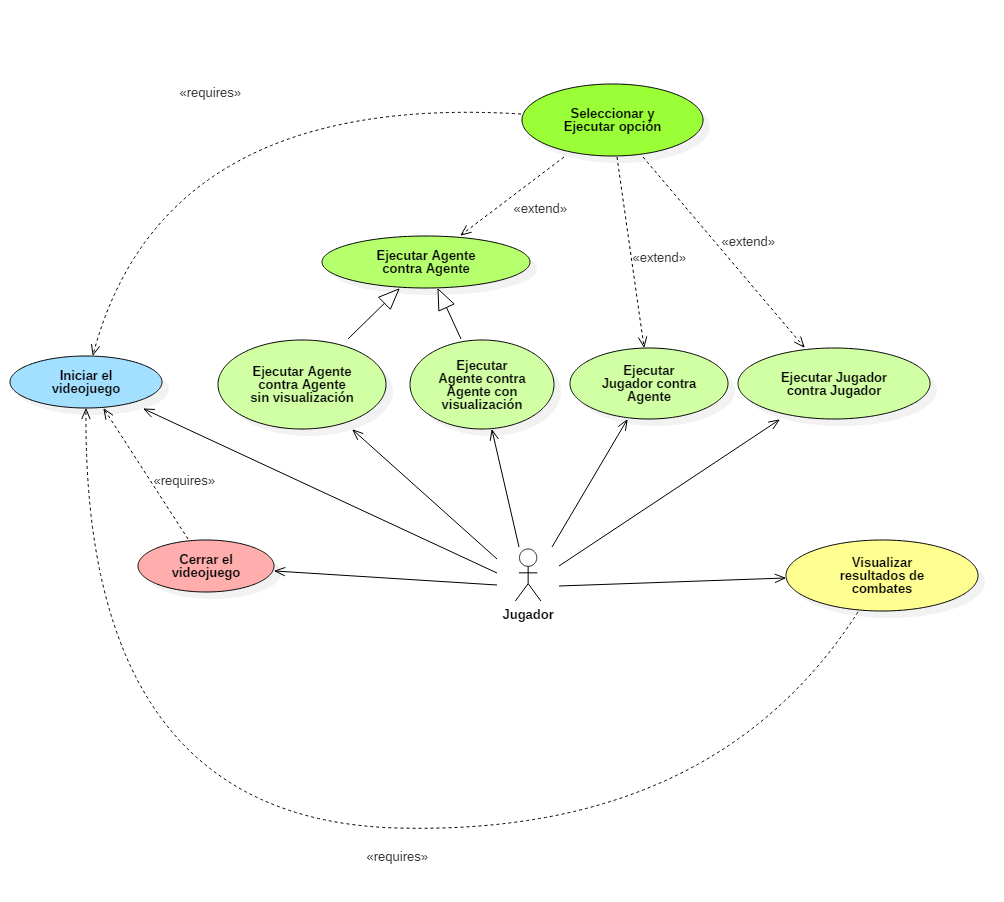
\includegraphics[width=10cm]{../diagramas/casosDeUsoCropped.png}}
	\label{casos_de_uso}
\end{figure}

\note{

}
\end{frame}

\subsection{Requisitos}
\begin{frame}
\frametitle{Requisitos}


\begin{columns}
	\begin{column}{5cm}
		
		
		\scalebox{0.75}{
		\begin{minipage}{2.0\linewidth}
		\begin{itemize}
			\item \textbf{RF-1/2/3}: Funcionalidades do menú
			\item \textbf{RF-4/15}: Consola con comandos/resultados
			\item \textbf{RF-5}: Saír da aplicación
			\item \textbf{RF-6}: Entrar na escena de combate
			\item \textbf{RF-7/8/9}: Moverse/Atacar/Defender
			\item \textbf{RF-10}: Gañar/Perder partida
			\item \textbf{RF-11}: Esgotar o tempo de combate
			\item \textbf{RF-12}: Volver ó menú
			\item \textbf{RF-13}: Visualizar combate entre axentes
			\item \textbf{RF-14}: Simular múltiples combates
		\end{itemize}
		\end{minipage}%
		}
	\end{column}
	\begin{column}{5cm}
			\scalebox{0.75}{
			\begin{minipage}{1.5\linewidth}
		\begin{itemize}
			\item \textbf{RNF-1}: Rendemento da aplicación
			\item \textbf{RNF-2}: \textbf{Velocidade das simulacións}
			\item \textbf{RNF-3}: Extensibilidade do motor
			\item \textbf{RNF-4}: Facilidade para depurar
			\item \textbf{RNF-5}: Aplicación autocontida
			\item \textbf{RNF-6}: Extensibilidade de escenas
			\item \textbf{RNF-7}: Documentación
			\item \textbf{RNF-8}: Usabilidade da interface
		\end{itemize}
	\end{minipage}%
}
	\end{column}
\end{columns}

\note{

}
\end{frame}

\section{Xestión do proxecto}

\subsection{Metodoloxía}
\begin{frame}
\frametitle{Metodoloxía}

\begin{block}{Contexto do proxecto}
\begin{itemize}
	\item Traballador único
	\item Duración relativamente corta
	\item Necesidade de avanzar rapidamente nas etapas iniciais
\end{itemize}
\end{block}

\begin{block}{Programación Extrema}
	\begin{itemize}
		\item Flexibilidade ante cambios
		\item Evitase utilizar demasiado tempo en tarefas de xestión
		\item Rápida iteración
		\item Reunións entre \textit{sprints}
	\end{itemize}
\end{block}

\note{

}
\end{frame}

\subsection{Planificación temporal}
\begin{frame}
\frametitle{Planificación temporal}

\begin{center}
\begin{tikzpicture}
	% squere, cloud
	\pie[sum=auto, after number={d}, cloud, radius = 2]{37/Videoxogo, 16/Axente, 3/Obtención de datos}
\end{tikzpicture}
\end{center}

\note{

}
\end{frame}

\section{Arquitectura}
\subsection{Arquitectura do sistema}
\begin{frame}
\frametitle{Subsistemas conectados}

\begin{figure}
	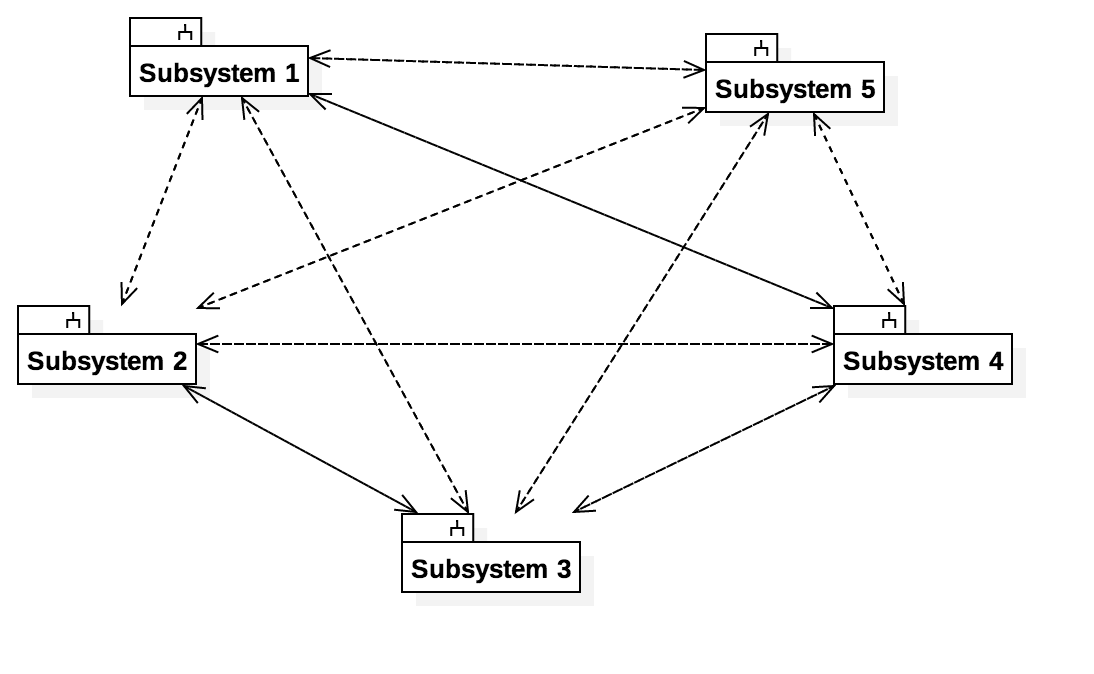
\includegraphics[width=10cm]{../otros/UML/png/arquitectura_mala.png}
	\label{dia:arquitectura_mala}
\end{figure}
\note{

}
\end{frame}
\begin{frame}
\frametitle{Bus de mensaxes}
\begin{figure}
	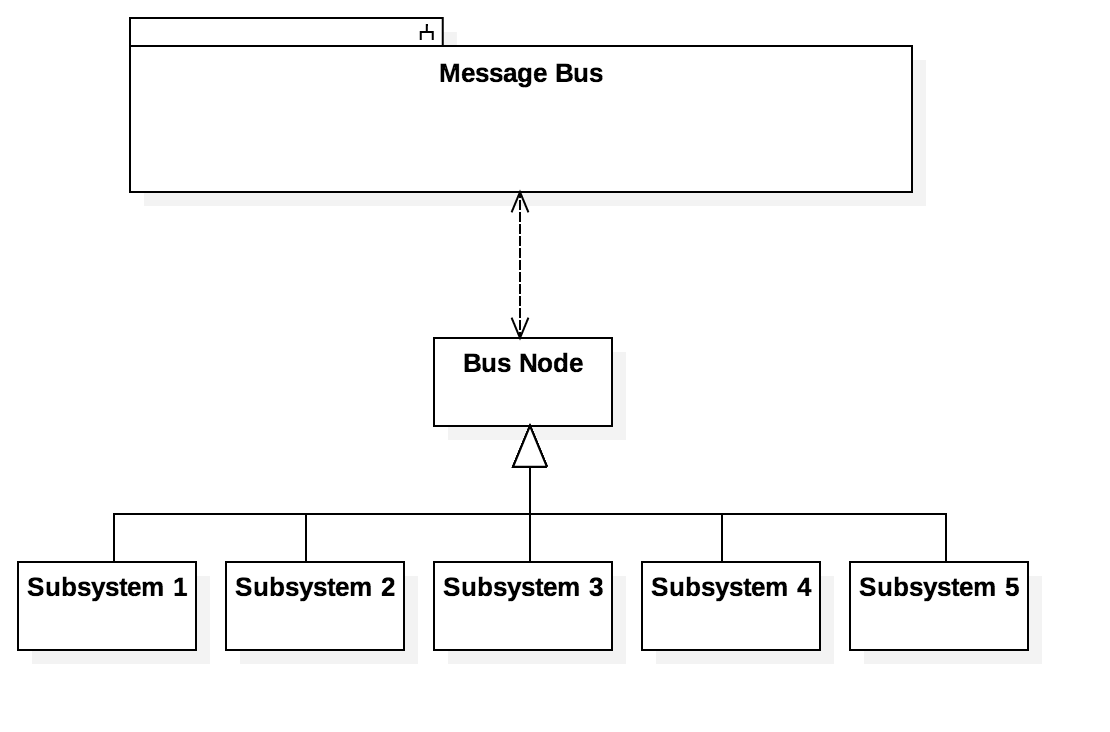
\includegraphics[width=10cm]{../otros/UML/png/actual_arquitecture.png}
	\label{dia:actual_arquitecture}
\end{figure}
\note{

}
\end{frame}
\begin{frame}
\frametitle{Arquitectura final}
\begin{figure}
	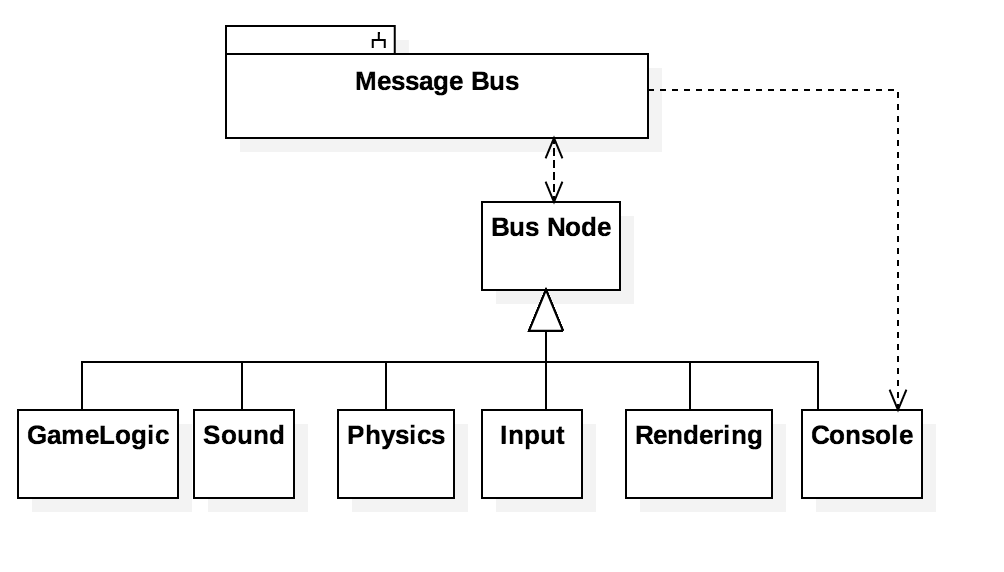
\includegraphics[width=10cm]{../otros/UML/png/final_arq.png}
	\label{dia:arquitectura_final}
\end{figure}
\note{

}
\end{frame}



% \section{Deseño}
% Agregar  o diagrama de clases do "GAME simplificado"

\section{Validación e probas}
\subsection{Aplicación}
\begin{frame}
\frametitle{Validación e probas da aplicación}
\begin{block}{Probas unitarias}
	Unha ou mais probas por cada requisito tanto funcional como non funcional superadas na sua totalidade.
\end{block}

\begin{block}{Probas de integración}
	Comproban a integración entre subsistemas e do o axente ca aplicación.
\end{block}
\note{

}
\end{frame}
\subsection{Validación do Axente}
\begin{frame}
\frametitle{Comparativa de vitorias}

\begin{figure}[h]
	\centerline{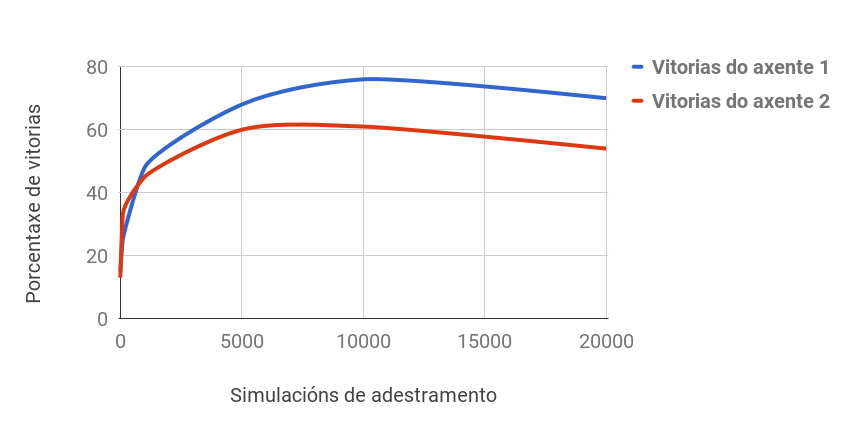
\includegraphics[width=11cm]{./graficos/vitorias.png}}
	\label{graf:victorias}
\end{figure}
\note{

}
\end{frame}

\begin{frame}
\frametitle{Comparativa de estados visitados}
\begin{figure}[h]
	\centerline{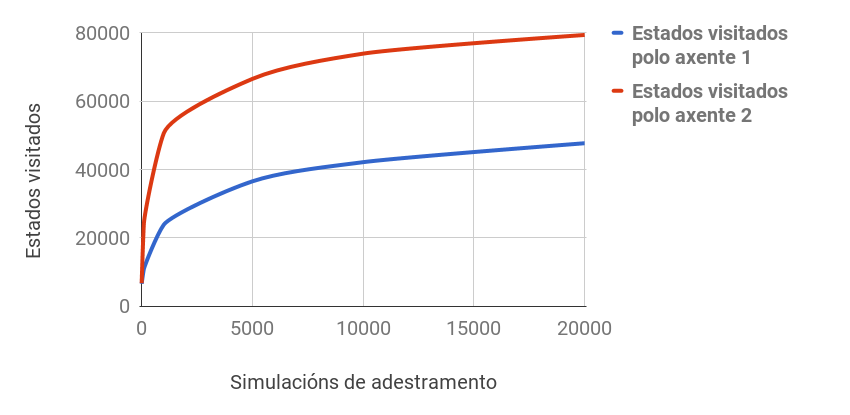
\includegraphics[width=11cm]{./graficos/estados.png}}
	\label{graf:estados}
\end{figure}

\note{

}
\end{frame}

\begin{frame}
\frametitle{Axente escollido}
Combinación de ámbolos dous métodos de adestramento.

\begin{block}{Contra o axente baseado en regras}
	Favorece un aprendizaxe moi rápido nas primeiras simulacións.
\end{block}

\begin{block}{Contra él mesmo}
	Aporta unha exploración de estados superior.
\end{block}
\note{

}
\end{frame}


\section{Conclusións}

\subsection{Conclusións e leccións aprendidas}
\begin{frame}
\frametitle{Conclusións e leccións aprendidas}
\begin{block}{Logros do proxecto}
\begin{itemize}
	\item O comportamento, aspecto e rendemento da aplicación cumpriu as expectativas.
	\item O axente é capaz de competir contra outras implementacións e contra xogadores humanos.
\end{itemize}
\end{block}

\begin{block}{Leccións aprendidas}
	\begin{itemize}
		\item Importancia de ter en conta os posibles riscos do proxecto o antes posible.
		\item Utilidade de un deseño flexible previo á implementación.
		\item Calidade dos resultados de implementacións sinxelas de Intelixencia Artificial.
	\end{itemize}
\end{block}

\end{frame}

\subsection{Posibles ampliacións}
\begin{frame}
\frametitle{Posibles ampliacións}
\begin{itemize}
	\item Melloras de compatibilidade.
	\item Ampliación do proceso de probas con xogadores humanos.
	\item Implementación de máis técnicas para o axente.
	\item Novas mecánicas para o videoxogo.
\end{itemize}

\end{frame}


% ========================= EXEMPLOS =========================  %
\begin{comment}
\section{Sección 1} 
\subsection{Ejemplo de subsección}
\begin{frame}
\frametitle{Título} 
Cada pantalla tiene su título.
\end{frame}

\subsection{Ejemplo de lista}

\begin{frame}
\frametitle{Lista no numerada}
\begin{itemize}
\item una  
\item dos 
\item tres 
\item cuatro
\end{itemize} 
\end{frame}

\begin{frame}
\frametitle{Lista con pausa}
\begin{itemize}
\item número uno \pause 
\item número dos \pause 
\item número tres \pause 
\item número cuatro
\end{itemize} 
\end{frame}

\subsection{Otro ejemplo de lista}
\begin{frame}
\frametitle{Lista numerada}
\begin{enumerate}
\item una  
\item dos 
\item tres 
\item cuatro
\end{enumerate}
\end{frame}

\section{Sección 2} 
\subsection{Tablas}

\begin{frame}
\frametitle{Tablas}
\begin{tabular}{|c|l|r|} \hline
\textbf{Centrado} & \textbf{Izquierda} & \textbf{Derecha} \\ \hline
AAAA  & 1000 & aaaa \\ \hline
BB    & 20   & bb \\ \hline
\end{tabular}
\end{frame}

\begin{frame}
\frametitle{Tabla con pausa}
\begin{tabular}{c c c}
A & B & C \\ \pause 
1 & 2 & 3 \\  \pause 
A & B & C \\ 
\end{tabular} 
\end{frame}

\section{Sección 3}
\subsection{Bloques}

\begin{frame}
\frametitle{Bloques}

\begin{block}{Bloque normal}
Texto del bloque normal
\end{block}

\begin{exampleblock}{Bloque de ejemplo}
Texto del bloque ejemplo
\end{exampleblock}

\begin{alertblock}{Bloque de alerta}
Texto del bloque alerta
\end{alertblock}
\end{frame}

\section{Sección 4}
\subsection{Pantalla dividida}

\begin{frame}
\frametitle{Pantalla dividida}
\begin{columns}
\begin{column}{5cm}
\begin{itemize}
\item una lista
\item de puntos 
\item mas una tabla 
\end{itemize}
\end{column}
\begin{column}{5cm}
\begin{tabular}{|c|c|c|} \hline
\textbf{Mes} & \textbf{Día} & \textbf{Hora} \\ \hline
Enero   & 10 & 15:30 \\ \hline
Febrero & 20 & 20:00 \\ \hline
\end{tabular}
\end{column}
\end{columns}
\end{frame}

\subsection{Figuras} 
\begin{frame}
\frametitle{Incluir figuras}
\begin{figure}

\includegraphics[scale=0.3]{../figuras/logo_usc.eps} 
\caption{Logo de la USC}
\end{figure}
\end{frame}

\subsection{Listas con figuras y pausas} 

\begin{frame}
\frametitle{Listas con figuras y pausas}
\begin{columns}
\begin{column}{4cm}
\begin{itemize}
\item<1-> Una
\item<3-> Dos
\item<5-> Tres
\end{itemize}
\vspace{3cm} 
\end{column}
\begin{column}{4cm}
\begin{overprint}
\includegraphics<2>[scale=0.05]{../figuras/logo_usc.eps}
\includegraphics<4>[scale=0.10]{../figuras/logo_usc.eps}
\includegraphics<6>[scale=0.15]{../figuras/logo_usc.eps}
\end{overprint}
\end{column}
\end{columns}
\end{frame}

\subsection{Cuando se necesita más espacio} 
\begin{frame}[plain]
\frametitle{Pantalla plana con sólo una figura}
\begin{figure}
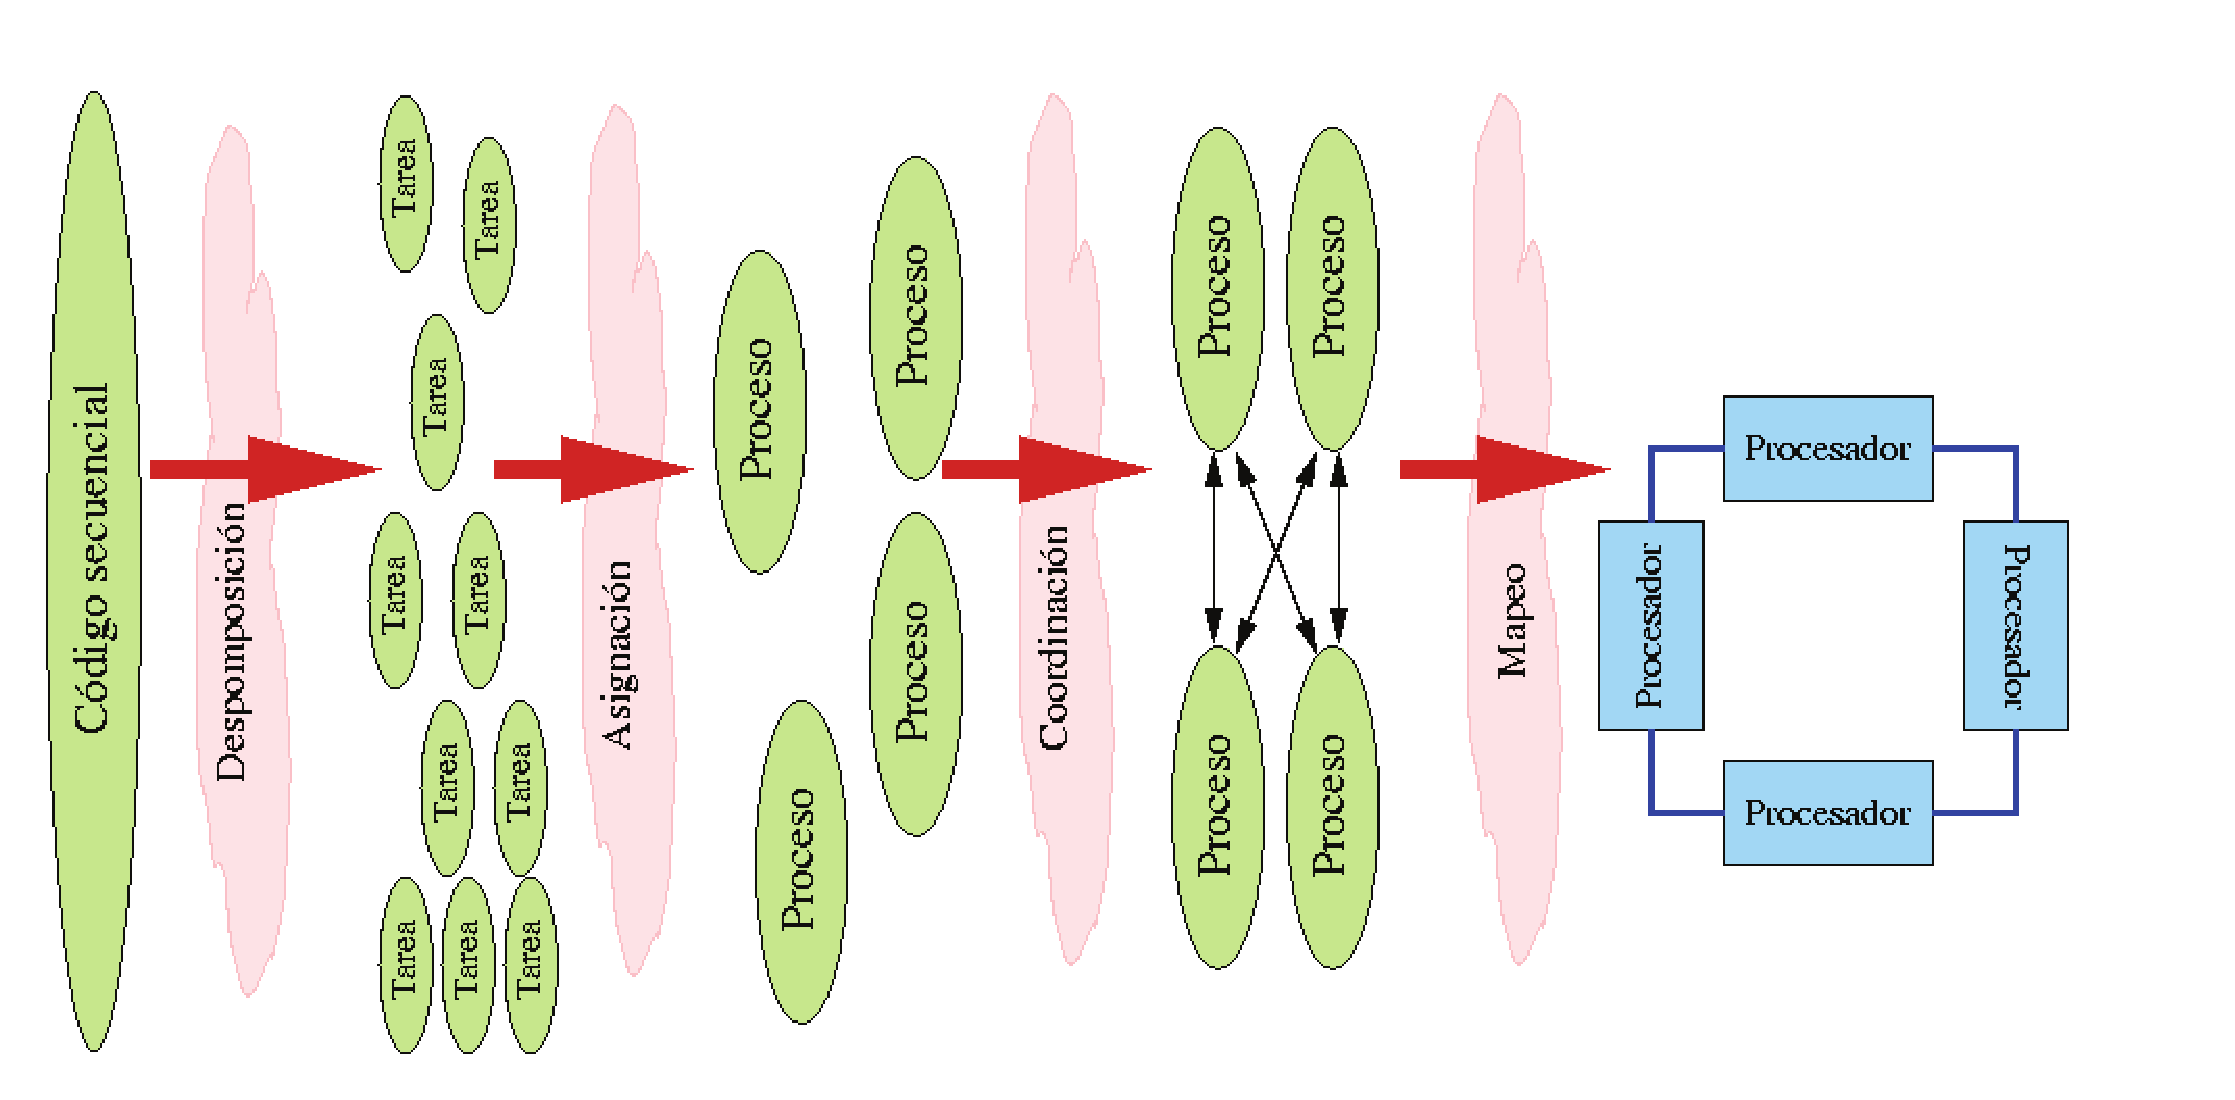
\includegraphics[scale=0.3]{../figuras/figura01.eps} 
\caption{Una figura grande}
\end{figure}
\end{frame}
\end{comment}

\end{document}

